\section{Poprawa jakości rozwiązania w algorytmach LS}
\subsection{Instancja br17.atsp}
\begin{figure}[!h]
\centering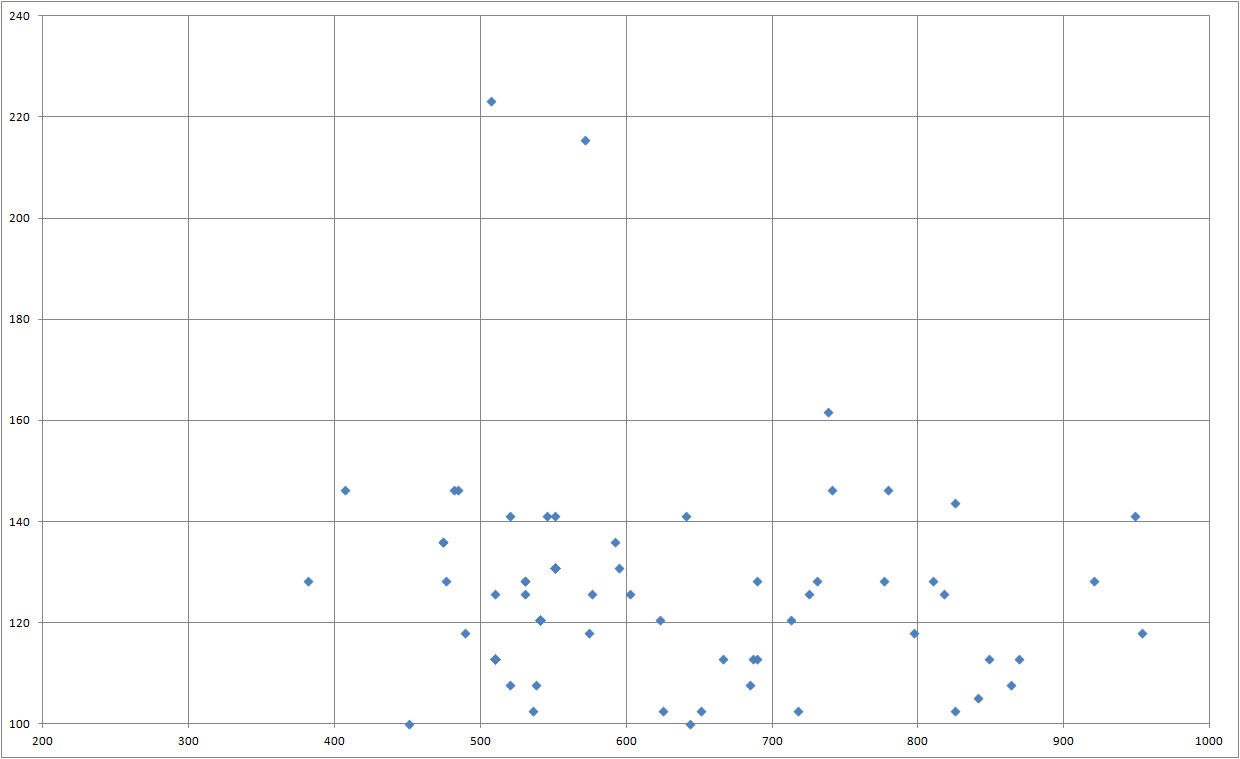
\includegraphics[width=12cm]{img/br17_b2e_g.png}
\caption{Poprawa jakości algorytmu Greedy dla instancji br17. Na osi pionowej odłożono procentowe wartości rozwiązania końcowego, na osi poziomej z kolei procentowe wartości rozwiązania startowego względem znanego optimum. Punkty przedstawiają poszczególne rozwiązania uzyskane przez kolejne odpalenia algorytmu dla tej samej instacji, lecz dla innych punktów startowych.}\label{rys:br17g}
\end{figure}
\begin{figure}[!h]
\centering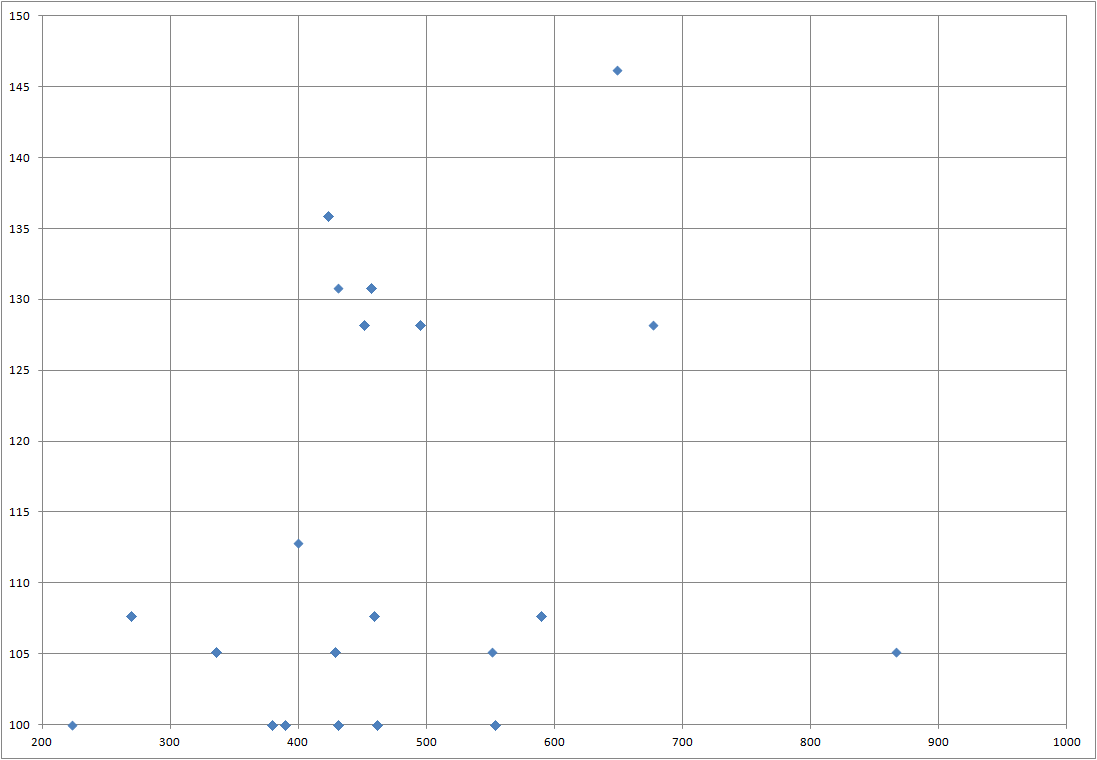
\includegraphics[width=12cm]{img/br17_b2e_s.png}
\caption{Poprawa jakości algorytmu Steppest dla instancji br17. Na osi pionowej odłożono procentowe wartości rozwiązania końcowego, na osi poziomej z kolei procentowe wartości rozwiązania startowego względem znanego optimum. Punkty przedstawiają poszczególne rozwiązania uzyskane przez kolejne odpalenia algorytmu dla tej samej instacji, lecz dla innych punktów startowych.}\label{rys:br17s}
\end{figure}

Dla tej instacji obydwa algorytmy zachowywały się dość ciekawie co zaprezentowano na rysunku \ref{rys:br17g} i \ref{rys:br17s}. Okazuje się, że Steppest znalazł kilkukrotnie rozwiązanie optymalne i zasadniczo znajdował lepsze rozwiązania niż Greedy. Można zauważyć, że taktyka przeskakiwania od razu do lepszego rozwiązania, a nie przeglądanie wszystkich sąsiadów dookoła jest dla tej instancji całkiem dobra, ponieważ prawie zawsze znajdowano rozwiązanie o conajwyżej 50\% gorsze od optimum. Dwa przypadki, kiedy algorytm Greedy nie zadziałał tak skutecznie świadczą o tym, że musiało istnieć pewne lokalne minimum, w które właśnie ten algorytm ma większą szansę wpaść aniżeli Steppest, ponieważ nie przegląda całego sąsiedztwa aktualnie analizowanego rozwiązania. Więc ma tendencje do zeskakiwania w złym kierunku (ku gorszemu minimum lokalnemu można by powiedzieć).

\subsection{Instancja ftv33.atsp}
\begin{figure}[!h]
\centering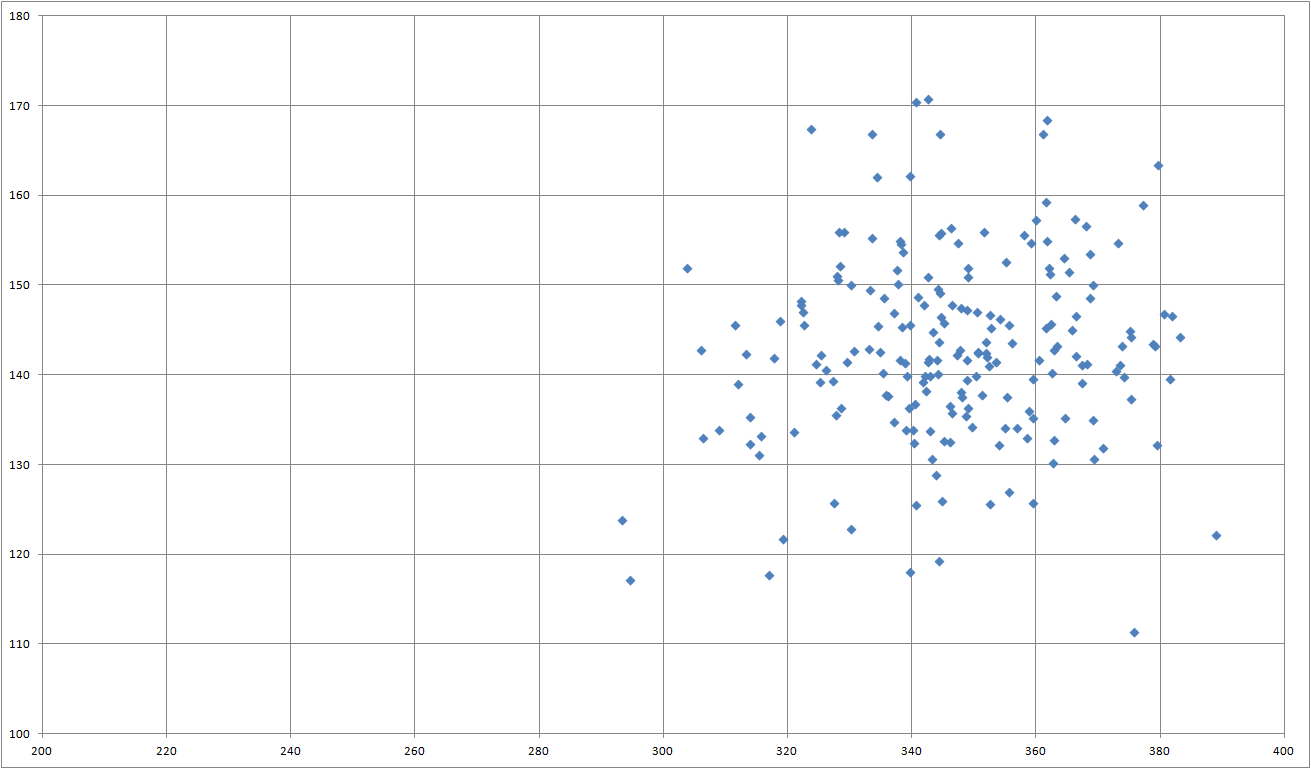
\includegraphics[width=12cm]{img/ftv33_b2e_g.png}
\caption{Poprawa jakości algorytmu Greedy dla instancji ftv33. Na osi pionowej odłożono procentowe wartości rozwiązania końcowego, na osi poziomej z kolei procentowe wartości rozwiązania startowego względem znanego optimum. Punkty przedstawiają poszczególne rozwiązania uzyskane przez kolejne odpalenia algorytmu dla tej samej instacji, lecz dla innych punktów startowych.}\label{rys:ftv33g}
\end{figure}
\begin{figure}[!h]
\centering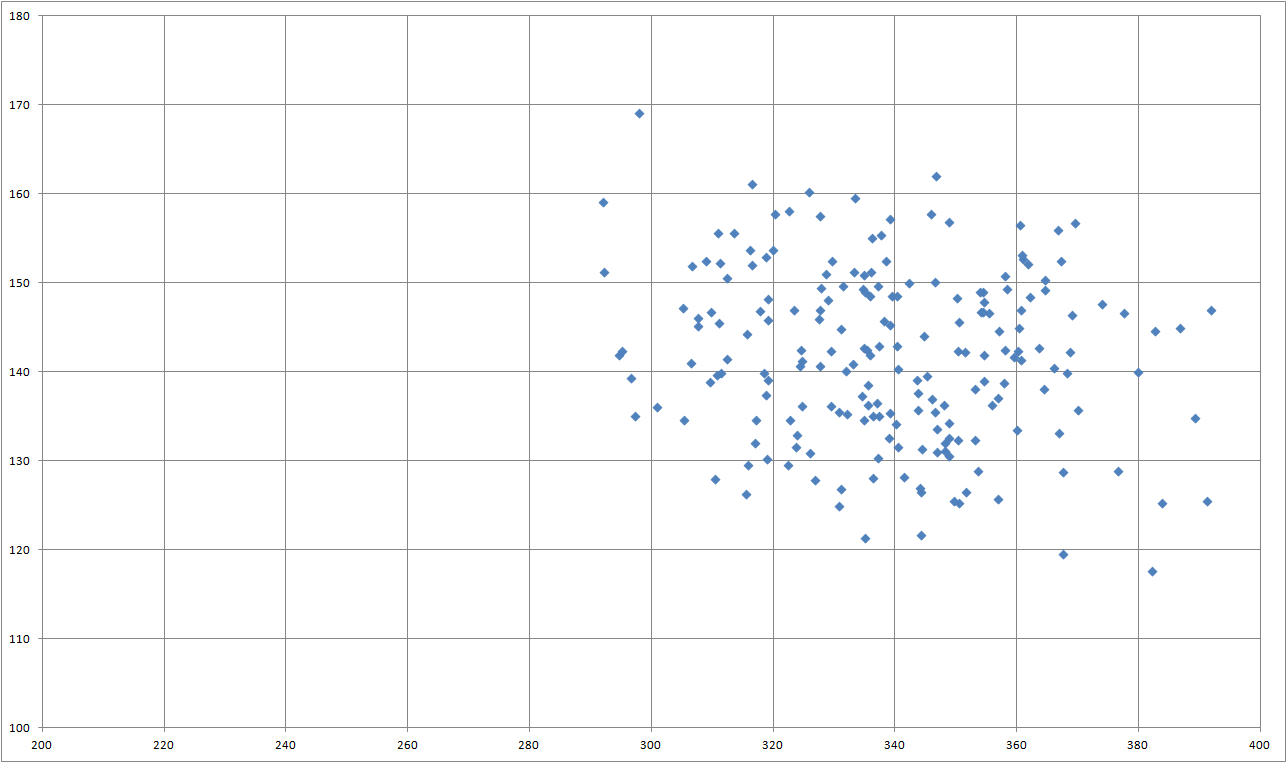
\includegraphics[width=12cm]{img/ftv33_b2e_s.png}
\caption{Poprawa jakości algorytmu Steppest dla instancji ftv33. Na osi pionowej odłożono procentowe wartości rozwiązania końcowego, na osi poziomej z kolei procentowe wartości rozwiązania startowego względem znanego optimum. Punkty przedstawiają poszczególne rozwiązania uzyskane przez kolejne odpalenia algorytmu dla tej samej instacji, lecz dla innych punktów startowych.}\label{rys:ftv33s}
\end{figure}

Ta instancja pokazuje przewagę dokładniejszego przeszukiwania sąsiedztwa przez algorytm Steppest nad pochopnym skakaniem do pierwszego znalezionego rozwiązania, które jest lepsze. Na rysunku \ref{rys:ftc33g} i \ref{rys:ftv33s} widać, że tendencja obydwu algorytmów jest bardzo podobna i odnajdują głównie rozwiązania odległe od optimum od 20\% do 50\%. Jednak co ciekawe algorytm Greedy jednak kilkukrotnie trafił na lepsze rozwiązania niż Steppest. A więc nie wpadł w pierwszy lepszy ''dołek'' tylko go ominął i trafił na lepszy zbiór rozwiązań.

\subsection{Wnioski dotyczące jakości rozwiązania względem liczby uruchomień algorytmu}
Powyższe dwa przykłady pokazują, że obydwa podejścia różnią się tolerancją na kształt krajobrazu rozwiązań. Algorytm Greedy ma większą łatwość w przeskakiwaniu lokalnych minimów, dzięki czemu może trafić na lepsze rozwiązania jeśli balansuje na krawędzi dwóch lokalnych minimów. Oczywiście jego skuteczność zależy od kolejności przeglądania sąsiadów i kształtu krajobrazu. Z kolei algorytm Steppest zawsze ''leci'' w ustalonym kierunku. Od początku obiera pewne minimum lokalne za swój cel i zasadniczo można powiedzieć, że jest w związku z tym bardziej deterministyczny (co szczególnie widać na rysunku \ref{rys:br17s}, gdzie większość punktów się bardzo pokrywa, stąd jest ich tam wizualnie mniej). Można też zauważyć, że uzyskana poprawa jakości rozwiązania dla danej instancji bez względu na wykorzystany algorytm okazuje się oscylować wokół podobnych wartości.